\documentclass{article}
\usepackage{graphicx} % Required for inserting images
\usepackage[margin=1in,footskip=0.25in]{geometry}

\newcommand{\pandocbounded}[1]{\begin{center}#1\end{center}}

\providecommand{\tightlist}{%
  \setlength{\itemsep}{0pt}\setlength{\parskip}{0pt}}

\title{cs-by-hand-format}
\author{Anna Arpaci-Dusseau}
\date{April 2026}

\begin{document}

\maketitle
\section{q2.py Binary
Representations}\label{q2.py-binary-representations}

As humans, we are used to counting in base 10, we have 10 distinct
digits: 0,1,2,3,4,5,6,7,8,9. When we parse a number, 1,431 for example,
we understand this value as being \[1*1000 + 4*100 + 3*10 +1\].
Effectively, each digit is a \emph{weight} applied to a power of 10.

Computers, naturally, however only have access to 2 distinct values LOW
(voltage) and HIGH. Thus, it is natural to represent values in
\textbf{base 2} when we are talking about data in computing systems.

To work with \textbf{base 2} or \textbf{binary}, the basic same idea of
weights and powers applies. However, now when we see a value 11011, we
should understand this to mean 1\emph{2\^{}4 + 1}2\^{}3 + 0\emph{2\^{}2
+ 1}2\^{}1 + 1 *2\^{}0.

To represent a decimal value in binary, work from left to right. Take
out the largest possible power of two from the decimal value, write a 1
in the corresponding digit, and continue to work until you reach the
``one's place''.

\pandocbounded{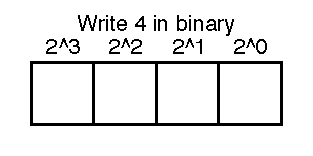
\includegraphics[keepaspectratio]{outputs/lec0-1/q2-1.pdf}}

\pandocbounded{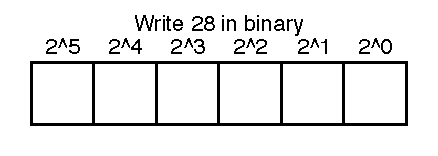
\includegraphics[keepaspectratio]{outputs/lec0-1/q2-2.pdf}}

\section{q1.py - 2's Complement
Circle}\label{q1.py---2s-complement-circle}

Now, what about negative values?

The most common convention to represent \textbf{signed integers} in
binary is 2's complement.

To represent a negative value in 2's complement: 1. Write the positive
version of the number in binary 2. Flip each digit (0-\textgreater1 or
1-\textgreater0) 3. Add 1 in binary (remember to carry if needed!)

Doing the procedure again (starting with a negative version of the
number in binary) will flip a negative value to a positive. Notice, that
positive values will always have a zero as the highest order bit, while
negative values will have a 1 in the highest order bit. As such, we call
the highest order bit, the \textbf{sign bit}. Consider: To represent the
value positive 4 in 2's complement, you will need 4 bits: 0100.

Fill in the circle with the decimal value of the following 4-bit 2's
complement binary around the circle.

\pandocbounded{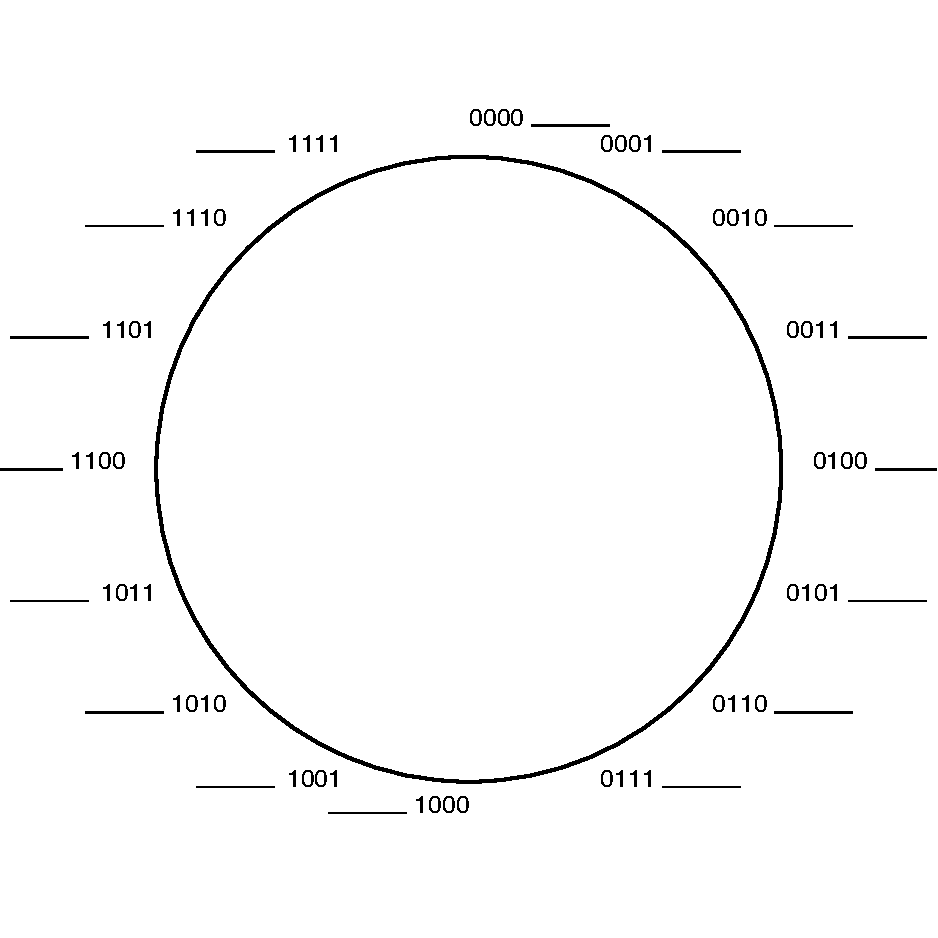
\includegraphics[keepaspectratio]{outputs/lec0-1/q1.pdf}}

Consider drawing arrows on the circle representing:

\begin{enumerate}
\def\labelenumi{\arabic{enumi}.}
\tightlist
\item
  Add 4 to 1.
\item
  Add 2 to -1.
\item
  Subtract 3 from 2.
\item
  Subtract 3 from -1.
\end{enumerate}

Notice how adding always goes clockwise around the circle and
subtracting goes counter-clockwise. 2's complement representation makes
binary arithmetic continuos, with no special cases for negatives,
positives, etc.

Except-- consider what happens when we add 3 to 6\ldots{}

This would result in \textbf{overflow} as we can not represent 9 in
4-bit 2's complement. Instead, the operation leaves us with a
representation of a negative value in 4-bit 2's complement.

\section{q2.py Binary Representations with
Negatives}\label{q2.py-binary-representations-with-negatives}

Write the following signed integer in 2's complement binary.

\pandocbounded{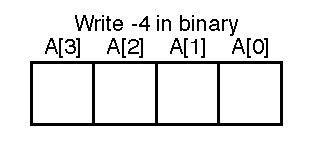
\includegraphics[keepaspectratio]{outputs/lec0-1/q2-3.pdf}}

\pandocbounded{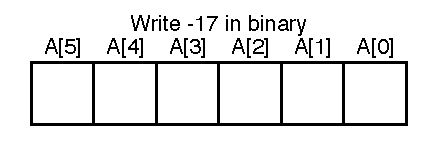
\includegraphics[keepaspectratio]{outputs/lec0-1/q2-4.pdf}}

\section{q3.py Binary Arithmetic}\label{q3.py-binary-arithmetic}

Consider we can also do arithmetic with binary values just as we can
with decimal values.

However, now when we do 1+1 in a single column, we must carry a 1 (from
the resulting 10), to the next column. (This is similar to how we would
carry a ``1'' to the tens place from adding 5+5 in decimal.)

\pandocbounded{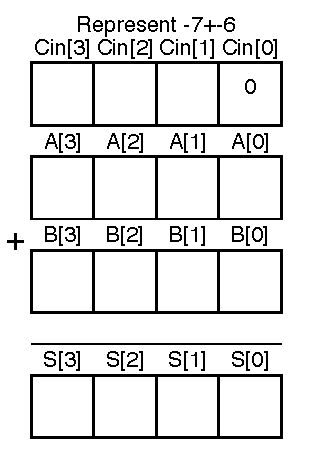
\includegraphics[keepaspectratio]{outputs/lec0-1/q3-1.pdf}}
\pandocbounded{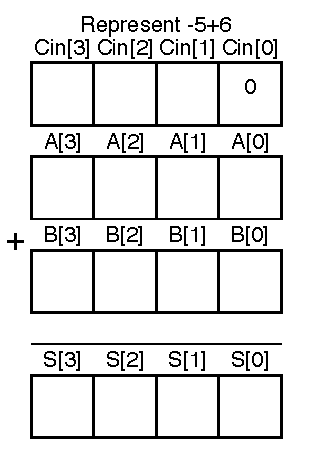
\includegraphics[keepaspectratio]{outputs/lec0-1/q3-2.pdf}}

\section{q4.py Hex/Binary Table}\label{q4.py-hexbinary-table}

Now, in computer systems it can become unwieldy and error-prone to
transcribe long binary values by hand! Furthermore, we have seen that
translating from decimal-\textgreater binary or vice versa requires a
bit of math.

However, let's now consider \textbf{base 16} or \textbf{hexidecimal}.
Why introduce a new base?

\begin{enumerate}
\def\labelenumi{\arabic{enumi}.}
\tightlist
\item
  Base 16, like base 10, has enough digits to be compact and easy for
  humans to read and write.
\item
  Base 16 has a nice property-- four binary digits correspond to exactly
  one hex digit. Thus, converting a binary value to hex is as simple as
  grouping digits into fours, and then a one-to-one translation!
\end{enumerate}

If you understand base 10 as the base for humans, and base 2 as the base
for computers, base 16 is the base for programmers (the middle man so to
speak)!

Complete the table below.

\pandocbounded{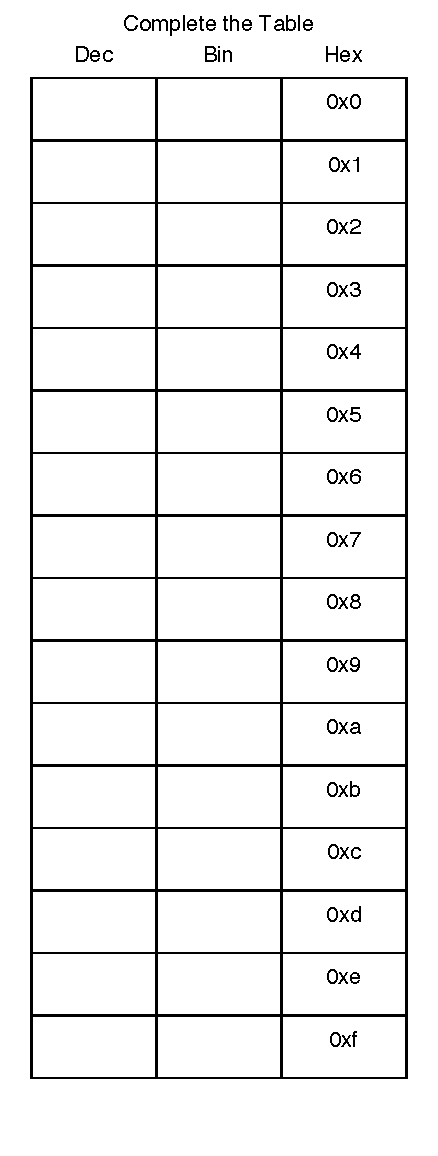
\includegraphics[keepaspectratio]{outputs/lec0-1/q4.pdf}}

\section{q5.py Hex Representation}\label{q5.py-hex-representation}

Complete the following binary-\textgreater hex conversions or
hex-\textgreater binary conversions. This should be far easier than
working with binary-\textgreater decimal for example!

\textbf{Hint:} Feel free to use the table you completed above.

\pandocbounded{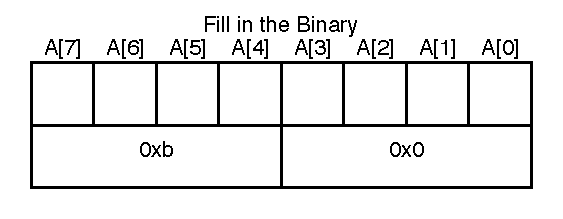
\includegraphics[keepaspectratio]{outputs/lec0-1/q5-1.pdf}}
\pandocbounded{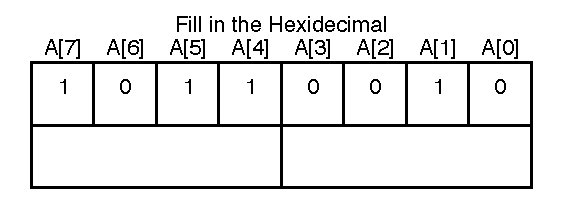
\includegraphics[keepaspectratio]{outputs/lec0-1/q5-2.pdf}}
\pandocbounded{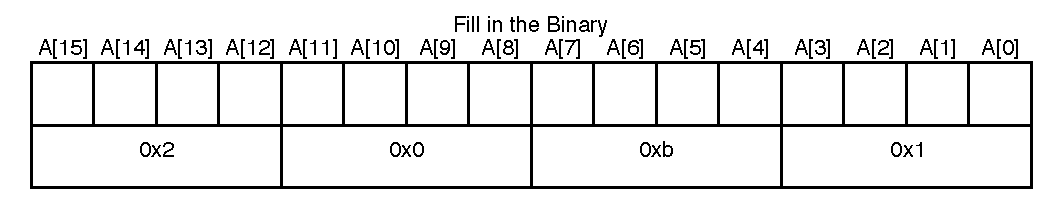
\includegraphics[keepaspectratio]{outputs/lec0-1/q5-3.pdf}}
\pandocbounded{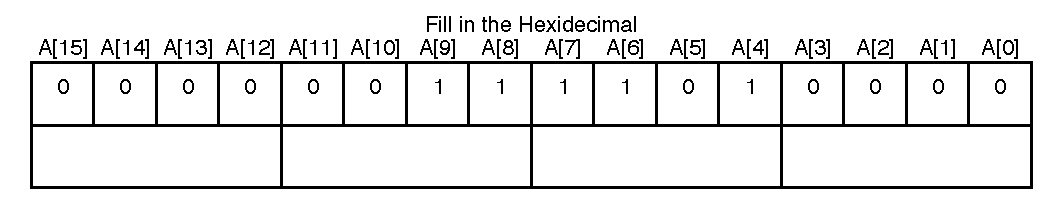
\includegraphics[keepaspectratio]{outputs/lec0-1/q5-4.pdf}}
\newpage
\subsection{q1.py SOP Expression}\label{q1.py-sop-expression}

\subsection{q2.py Logic Gates and Truth
Tables}\label{q2.py-logic-gates-and-truth-tables}

A fundamental computer of computer circuitry is the logic gate. Logic
gates take in two signals (HIGH/LOW voltages) and output a HIGH or LOW
signal in turn.

In this section, we will see how we can combine this gates to do
complicated functions, like adding, storage, etc, and build up to a
complete CPU (computer brain!).

Below, we have:

\begin{enumerate}
\def\labelenumi{\arabic{enumi}.}
\tightlist
\item
  AND (produces a 1 if A and B are 1. Otherwise 0)
\item
  OR (produces a 1 if either A and B, or both, are 1. Otherwise 0.)
\item
  XOR (produces a 1 if either, but not both, A and B are 1. Otherwise
  0.)
\item
  NAND (not and) (produces a 1 if A and B are 0. Otherwise 1)
\item
  NOR (not or) (produces a 0 if either A and B, or both, are 1.
  Otherwise 1.)
\item
  NOT XOR (produces a 0 if either, but not both, A and B are 1.
  Otherwise 1.)
\end{enumerate}

The final gate takes is one input, and produces one output.

\begin{enumerate}
\def\labelenumi{\arabic{enumi}.}
\setcounter{enumi}{6}
\tightlist
\item
  Inverter (not) (if A is 1, produces 0. Otherwise 1.)
\end{enumerate}

We can represent logical statements as truth tables.

On the left side of the bolded truth table line, fill in all the
possible input values for A and B. - done effectively, this will look
like counting in binary: A=0,B=0 (00), A=0,B=1 (01), A=1\ldots{} On the
right side of the bolded line, fill in the output given the
corresponding A and B values.

\pandocbounded{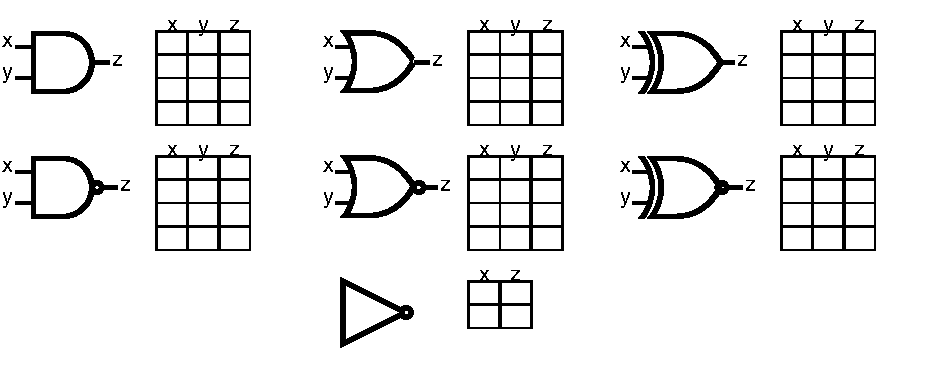
\includegraphics[keepaspectratio]{outputs/lec2/q2.pdf}}

\subsection{q3.py Truth Table, SOP, Draw the
circuit}\label{q3.py-truth-table-sop-draw-the-circuit}

Now, any logic table can be expressed as a ``sum of products expression
(SOP)''. In turn, any SOP expression can be represented in circuitry!
Thus, any truth table can be turned into a circuit.

For a given truth table, inspect each row. Say, that row 1, row 3, and
row 4 output TRUE (1).

Effectively, the entire truth table can be described as:

output = (condition for row 1) OR (condition for row 3) OR (condition
for row 4)

Then, each condition is simply the AND of each variable. For example if
we have A=1,B=0,C=1, we can describe that condition as

\[A\bar{B}C\]

Note, that OR is often represented by addition: \(+\), AND is
represented via multiplication \(\cdot\), and NOT is often represented
by a bar \(\bar{A}\).

\pandocbounded{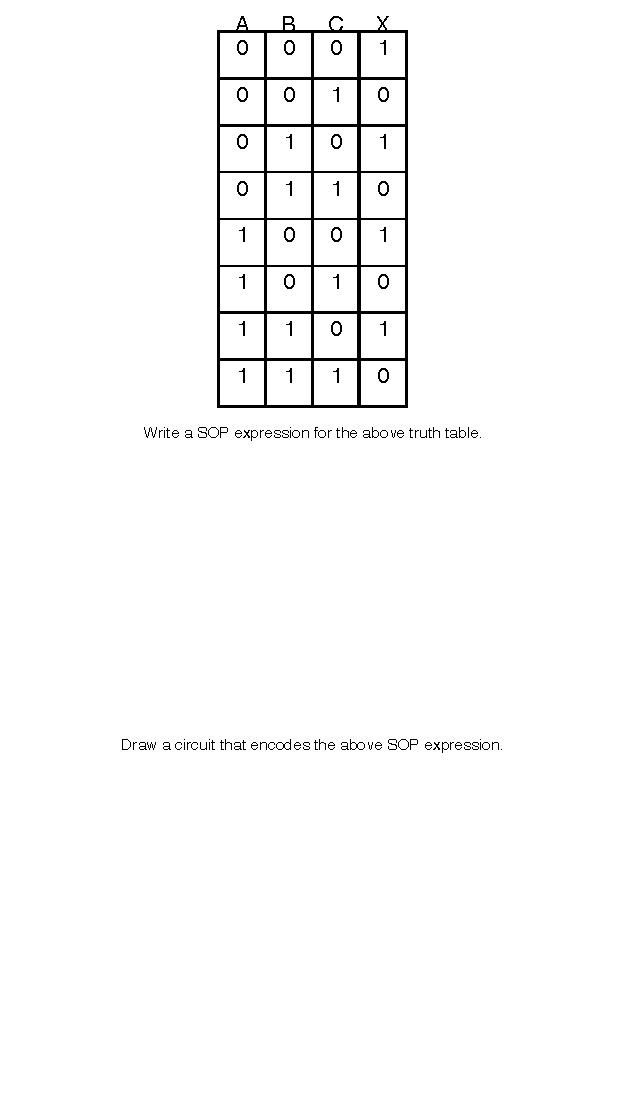
\includegraphics[keepaspectratio]{outputs/lec2/q3.pdf}}

\subsection{q4.py Timing Delays}\label{q4.py-timing-delays}

Now, circuits are real-world components. Like all real-world processes,
they take time to run and compute!

How long? Each circuit module has a timing specification described in
two parts:

Tpd is the \textbf{propagation delay} which means the time it takes from
giving input to getting correct output.

Tcd is the \textbf{contamination delay} which means the time it takes
from giving input to getting some incorrect (contaminated) reading.

Effectively, when building a circuit and combining modules, after giving
new input, after the contamination delay elapses we do not want to read
from the output until the propagation delay has passed.

\begin{enumerate}
\def\labelenumi{\arabic{enumi}.}
\tightlist
\item
  To calculate Tpd, find the longest path of summed Tpds of each
  component, along the path form input-\textgreater output.
\item
  To calculate Tcd, find the shortest path of summed Tcds of each
  component, along the path form input-\textgreater output.
\end{enumerate}

\pandocbounded{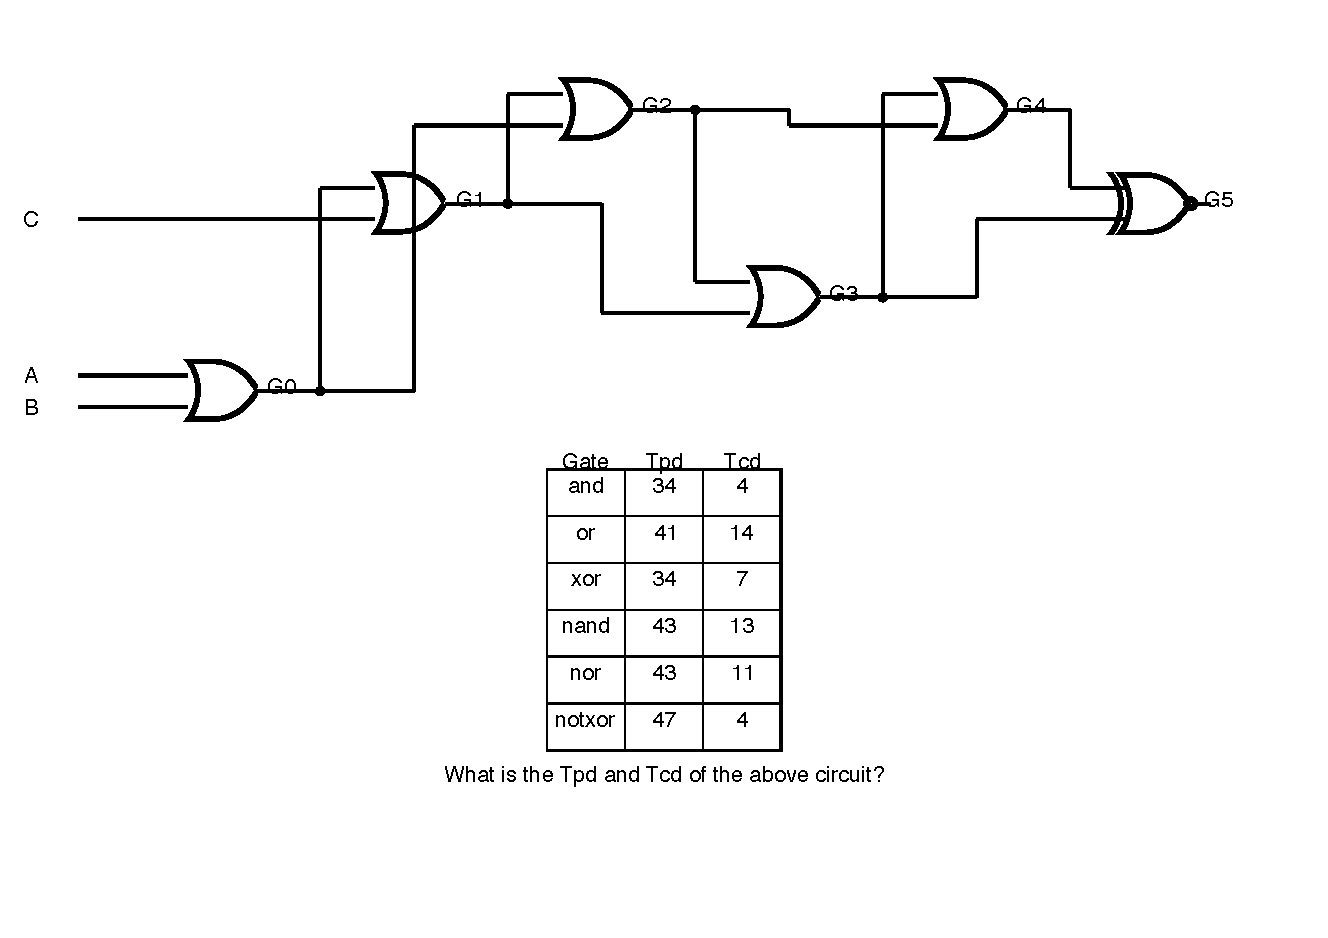
\includegraphics[keepaspectratio]{outputs/lec2/q4.pdf}}

\subsection{q5.py Control circuits-- MUX Truth Table,
Implementation}\label{q5.py-control-circuits-mux-truth-table-implementation}

Now, a common control component that will be useful for us is known as
the ``multiplexer''.

A 2-way multiplexer takes in two inputs, and uses a third input, a
``select bit'' to indicate if we want the output to be the 0th input
(S=0) or the 1st input (1st, S=1).

A n-way multiplexer takes in N inputs, and \texttt{ceil(log\_2(N))}
select bits to describe which of the N inputs to chose from.

\pandocbounded{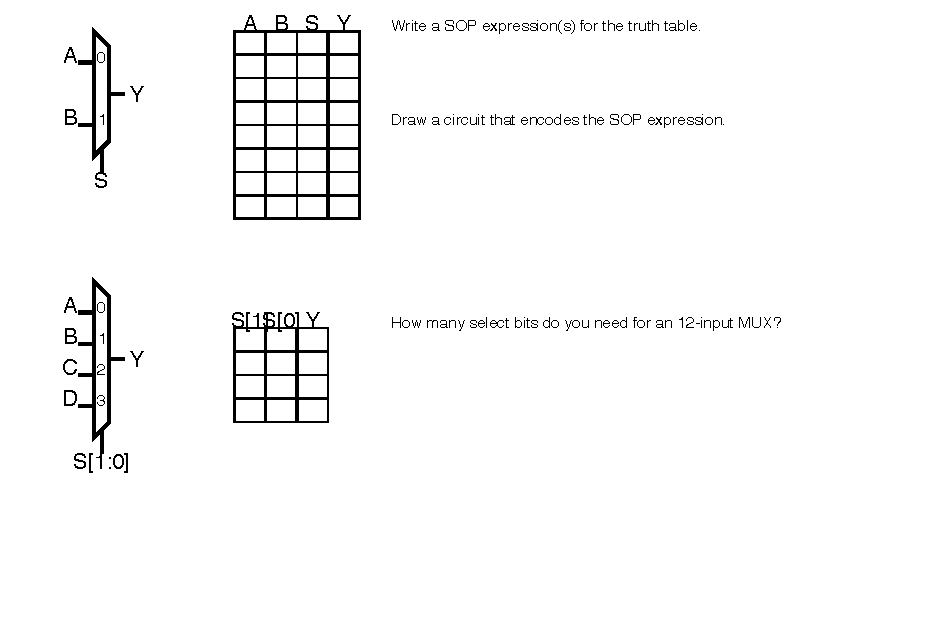
\includegraphics[keepaspectratio]{outputs/lec2/q5.pdf}}

\subsection{q6.py Full Adder}\label{q6.py-full-adder}

Now, remember from the last section how we did binary arithmetic. Can we
represent that operation in circuitry?

First, we must break down and understand the operation between three
1-bit values, A and B and the carry-in bit (Cin). What are the possible
outputs for S (the output value) and Cout (the carry out bit).

Just as before, we can represent this scenario as a truth table, then an
SOP expression, and then a circuit.

\pandocbounded{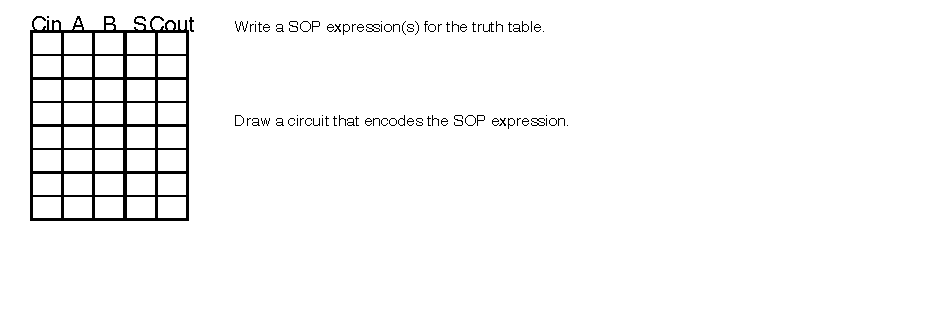
\includegraphics[keepaspectratio]{outputs/lec2/q6.pdf}}

\subsection{q7.py 4-bit full adder}\label{q7.py-4-bit-full-adder}

Now, consider, can be combine this full-adder module into a 4-bit adder?
To do so, we will build the conceptually simple (and slightly
inefficient) \textbf{ripple carry adder}. This adder will work by first
doing a 1-bit addition on A{[}0{]} and B{[}0{]}, producing S{[}0{]} and
then a carry out bit. This will be passed along to the next full adder
module to calculate A{[}1{]},B{[}1{]} and so on and so forth.

\pandocbounded{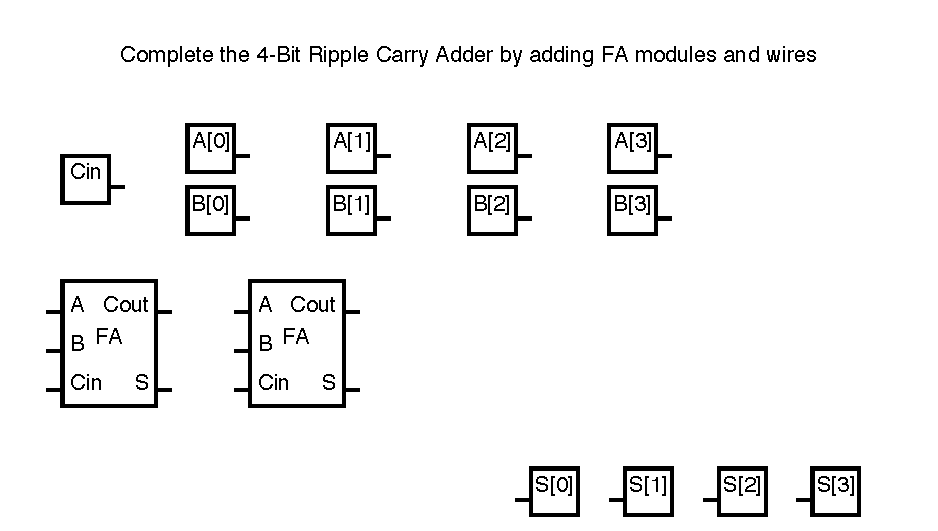
\includegraphics[keepaspectratio]{outputs/lec2/q7.pdf}}
\newpage
\subsection{q1.py Sequential Logic}\label{q1.py-sequential-logic}

Now, we must consider how can we ``remember'' or store information in
our circuitry. Computation is great! But to truly make a computer, we
must also have \textbf{stateful circuits} or circuits with ``memory''!

In order to represent stateful circuits, we will create circuits with
feedback loops.

Inspect the circuit below.

Consider the labeled signal 0. What is the value on all other wires in
the circuit?

\pandocbounded{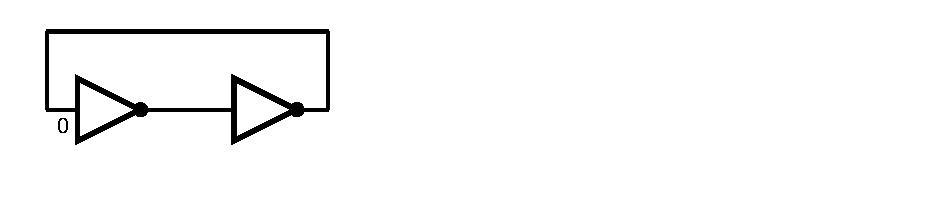
\includegraphics[keepaspectratio]{outputs/lec3/q1.pdf}}

Building off such ``feedback'' loops we can create stable storage.

\subsection{q2.py D-Latch Truth Table}\label{q2.py-d-latch-truth-table}

Create a feedback loop, draw a wire connecting Q to Q' in the schematic
below. This is a D-Latch.

Note, that we have labeled the ``select bit'' of the mux ``WE''. ``WE''
stands for write-enable. Does this make sense?

Now, fill out the truth table accordingly.

\pandocbounded{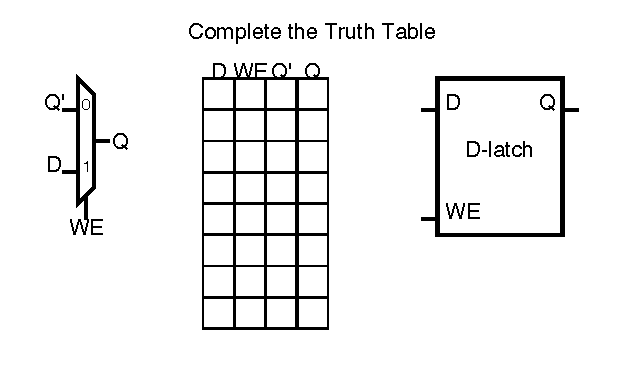
\includegraphics[keepaspectratio]{outputs/lec3/q2.pdf}}

We will represent the mux with feedback loop as the module ``D-Latch''
with inputs D and WE, and output Q.

\begin{enumerate}
\def\labelenumi{\arabic{enumi}.}
\tightlist
\item
  Which signal is the input data to write to the storage?
\item
  Which signal is the stored data value?
\end{enumerate}

\subsection{q3.py Flip Flop - Draw the
Waveform}\label{q3.py-flip-flop---draw-the-waveform}

The next question is a bit tricky. You may have noticed from the
previous sections that circuits are timing dependent! We must carefully
consider, how long does some particular output take to calculate.

In turn, enabling data to be stored, and then knowing when to read said
data is also a question of timing. When is a d-latch taking in new
inputs? Anytime WE is enabled! When is a d-latch emitting a new stable,
output? After WE is flipped, the duration of the tpd of a mux.

Building circuits around this timing consideration can be troublesome.
Instead, we find in practice, it is better to have \textbf{clocked
storage}. Modern circuits have access to an oscillating clock signal.
What if we could take in new inputs on the rising edge of a clock
instead? Then, we can read stable values from our storage at any clock
high?

Investigate the implementation of the flip flop below and complete the
missing waveforms given the CLK and input data.

\pandocbounded{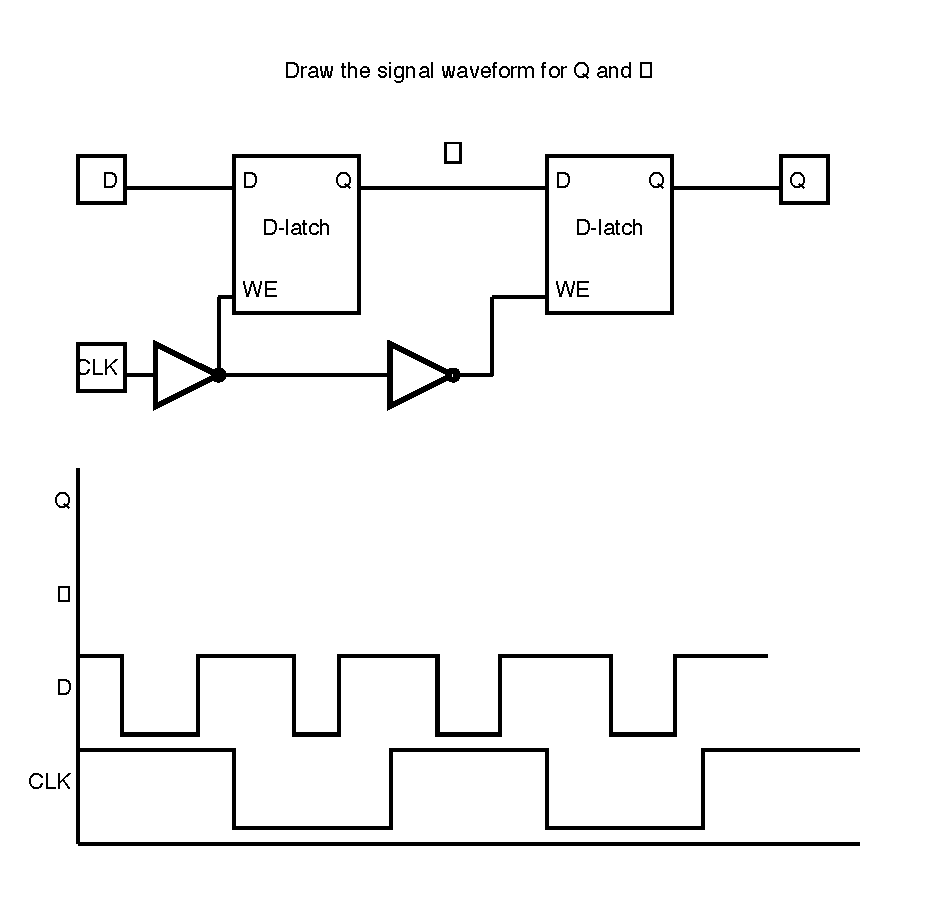
\includegraphics[keepaspectratio]{outputs/lec3/q3.pdf}}

\subsection{q4.py FSM -- Binary Combination
Lock}\label{q4.py-fsm-binary-combination-lock}

\pandocbounded{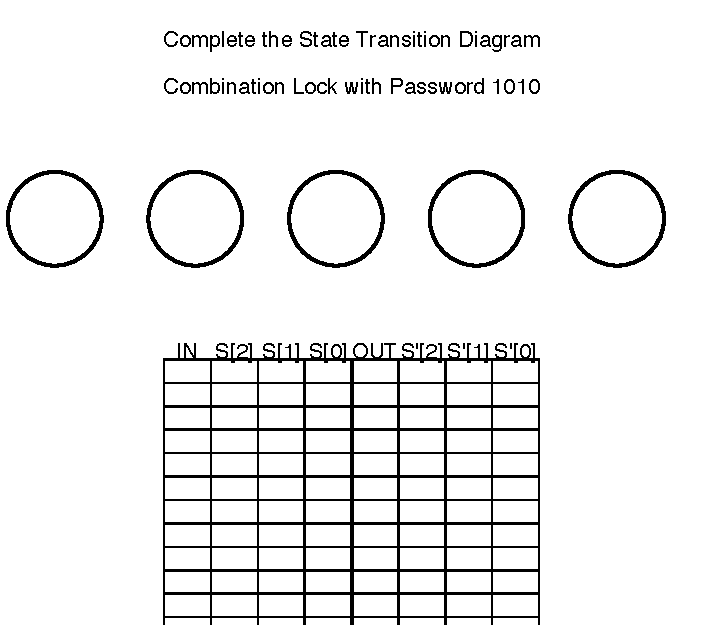
\includegraphics[keepaspectratio]{outputs/lec3/q4.pdf}}
\newpage
Now we will start to build up to constructing a full mini computer
processor that can perform 2 operations: addition and subtraction.

\section{q3.py - Full 4-bit Arith Unit for
ADD/SUB}\label{q3.py---full-4-bit-arith-unit-for-addsub}

Remember the 4-bit full adder you implemented in lec2.q7? We want to
expand the logic of the 4-bit adder to be a full ``arith'' unit.

This unit should use the 4-bit adder to perform addition, if the ALU bit
is 0. The unit should use the 4-bit adder to preform 2's-complement
subtraction if the ALU bit is 1.

Eventually, we will also want to use this arith unit to perform
comparison, for example. To do so, we will also compute 3 1-bit outputs,
called ``flag'' bits.

\begin{itemize}
\tightlist
\item
  The ``Z'' flag should be 1 if your four-bit output is equal to 0000.
\item
  The ``N'' flag should be 1 if your four-bit output is negative in 2's
  complement.
\item
  The ``V'' flag should be 1 if overflow occured.
\end{itemize}

The logic for this is equivalent to:
\[V = XA_{3} * XB_{3} * \overline{S_{3}} + \overline{XA_{3}} * \overline{XB_{3}} * S_{3}\]

Consider, how can we use SUB and this Z bit to check if two values are
equal? \_\_\_\_\_\_\_\_\_\_\_\_\_\_\_

Complete the implementation of the 4-bit arith unit below.

\pandocbounded{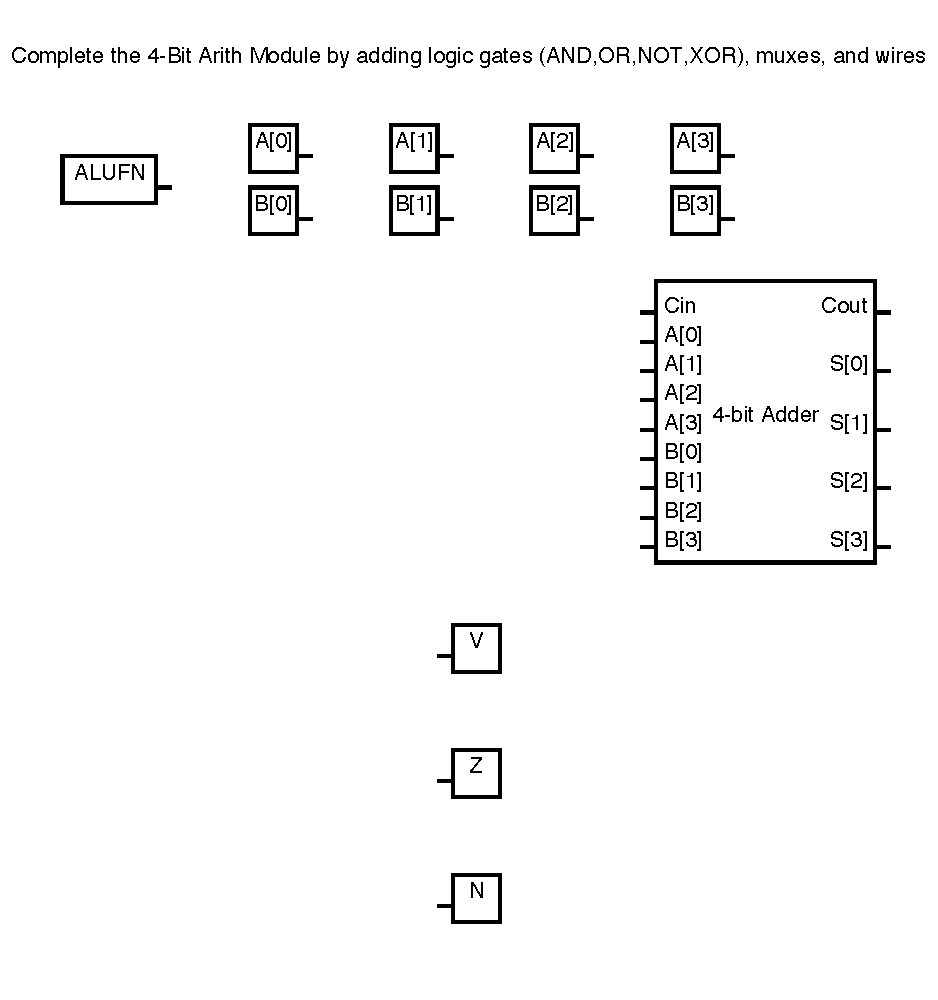
\includegraphics[keepaspectratio]{outputs/lec4/q3.pdf}}

\section{q1.py - mini computer for
N!}\label{q1.py---mini-computer-for-n}

Let's create a mini computer that can compute \(N!\).

To complete this task you will be creating two things:

\begin{itemize}
\tightlist
\item
  \textbf{The Data path}-- wires, muxes, registers, etc. that combine to
  move the data of our computation from our two computation modules
  (multiplication and -1).
\item
  \textbf{The Control path} -- when should our computation stop? To do
  this, you can compute a control signal as input to our control logic
  module. This control logic module can implement a finite state machine
  and output any needed \emph{control signals}, which our circuit can
  use as input.

  \begin{itemize}
  \tightlist
  \item
    Consider, that the registers' write enable signals should likely be
    output of our control logic.
  \end{itemize}
\end{itemize}

Complete the circuit by adding wires, registers, and control logic
description.

\pandocbounded{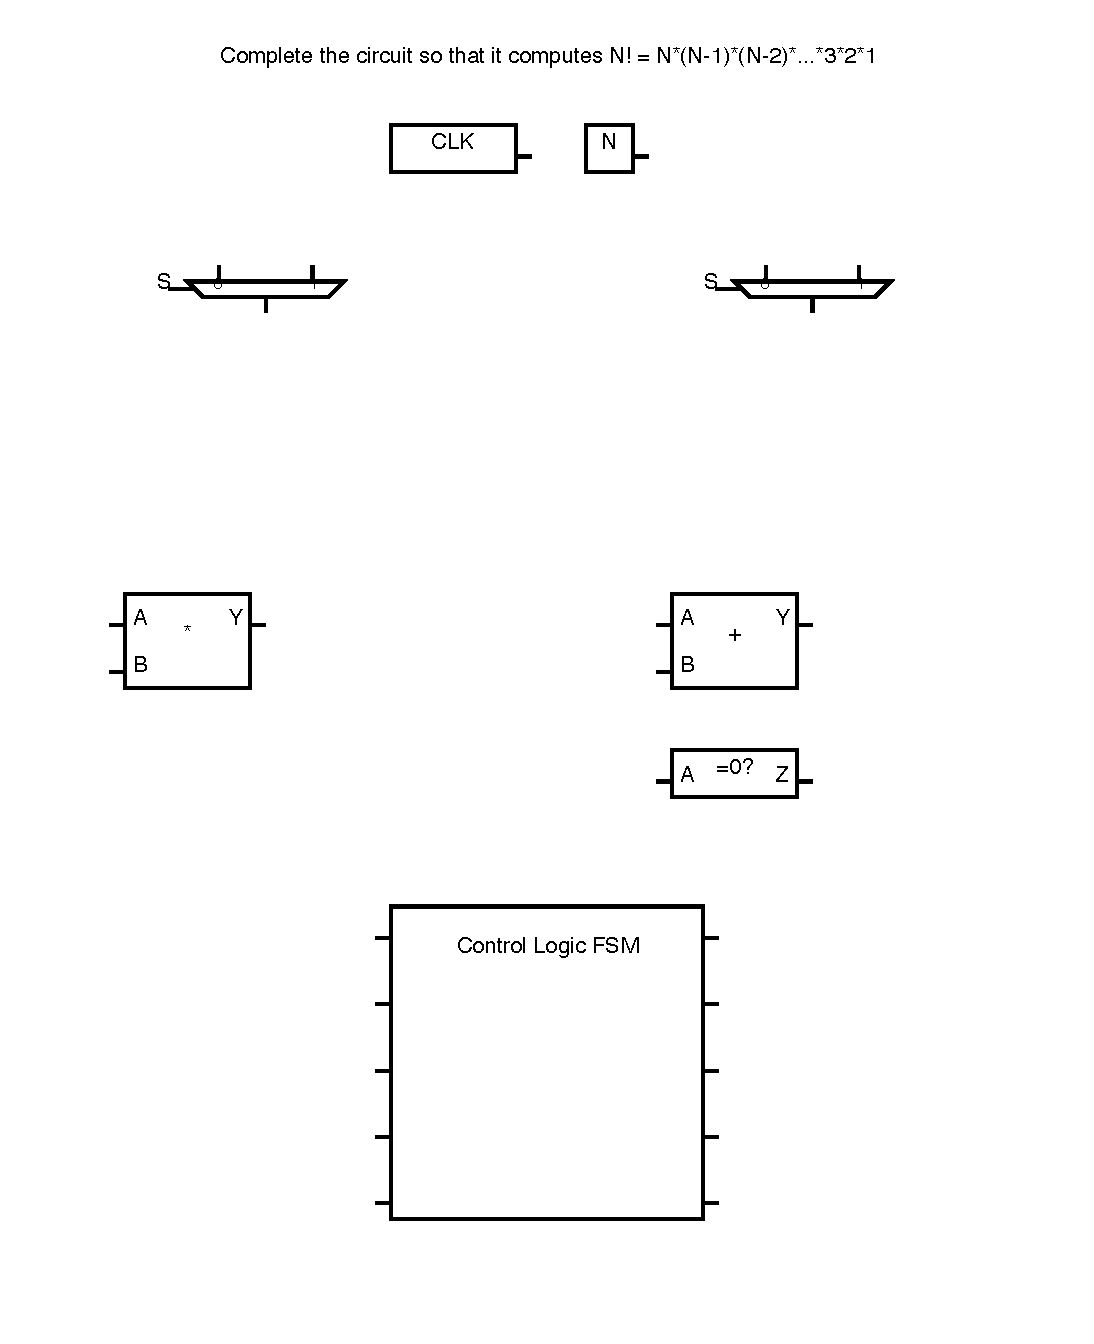
\includegraphics[keepaspectratio]{outputs/lec4/q1.pdf}}

\section{q2.py - mini general purpose 4-bit computer w/ instruction
memory?
(zero/add)?}\label{q2.py---mini-general-purpose-4-bit-computer-w-instruction-memory-zeroadd}

\begin{itemize}
\tightlist
\item
  Fetch, Decode, Execute
\item
  1 register
\item
  Arith Unit
\item
  Program Counter
\item
  Instruction Memory
\item
  CLK
\end{itemize}

\begin{verbatim}
ZERO
ADD 0
ADD 3
ADD -3
\end{verbatim}

\pandocbounded{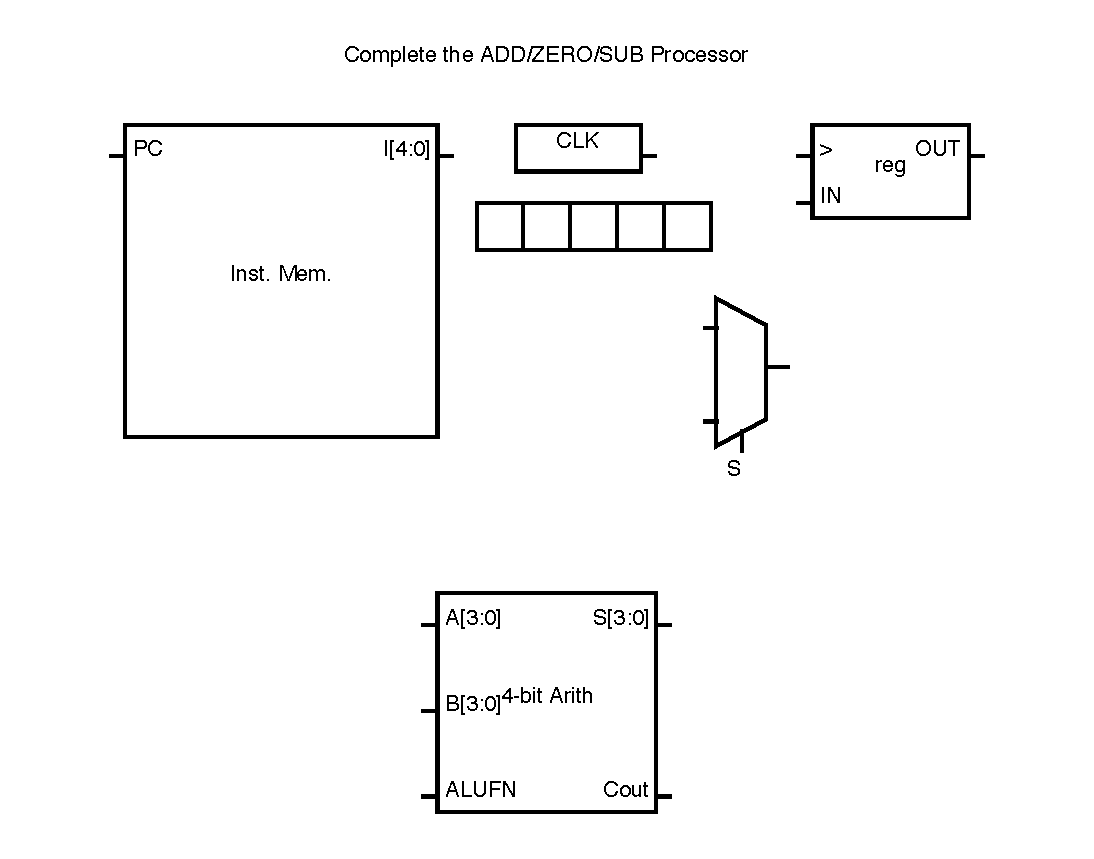
\includegraphics[keepaspectratio]{outputs/lec4/q2.pdf}}

\begin{itemize}
\tightlist
\item
  Draw the wires to compelte the mini-computer
\item
  Highlight the ``control path'', highlight the ``data'' path.
\item
  What must CLK cycle be set to?
\end{itemize}

\section{q4.py - add subtraction
operation?}\label{q4.py---add-subtraction-operation}

\begin{itemize}
\tightlist
\item
  1 register
\item
  Arith Unit w/ subtraction logic, new control signal for ALUFN
\item
  Program Counter
\end{itemize}

\begin{verbatim}
ZERO
ADD 0
ADD 3
SUB 2
ADD -3
\end{verbatim}

\pandocbounded{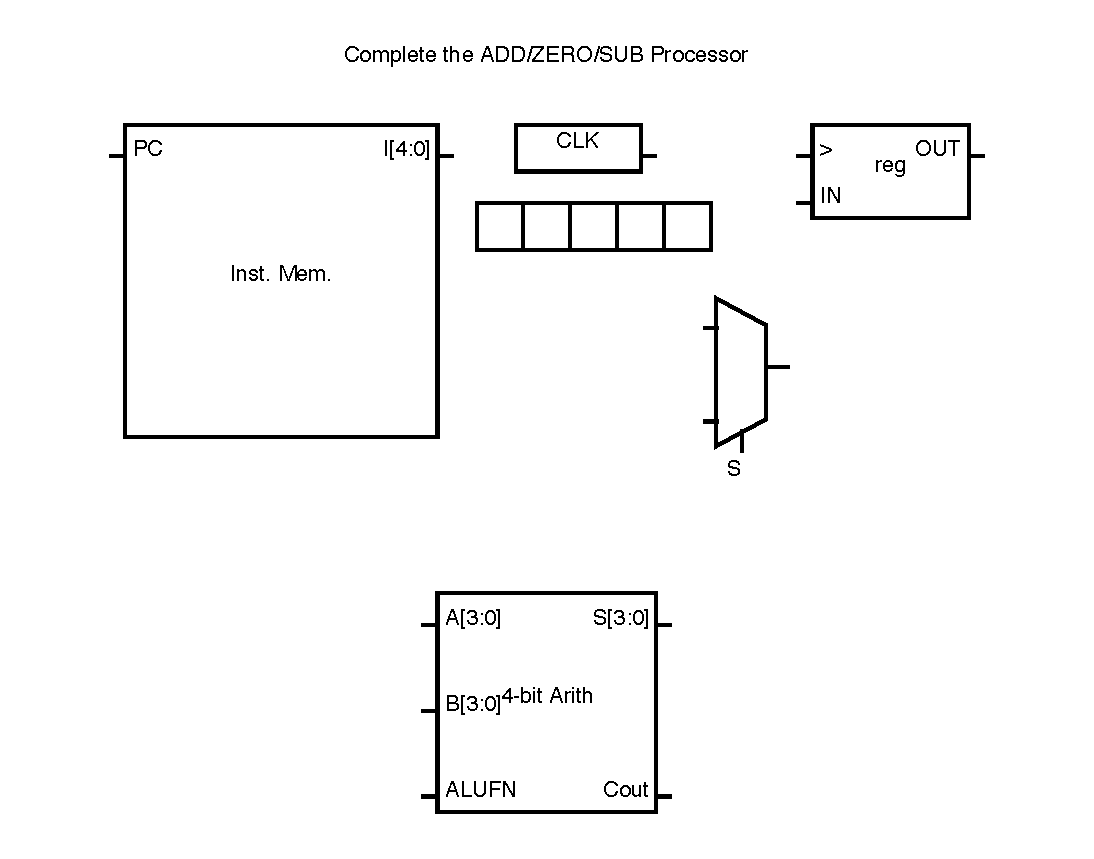
\includegraphics[keepaspectratio]{outputs/lec4/q2.pdf}}
\newpage
\end{document}